\documentclass[main.tex]{subfiles}
\begin{document}
\begin{enumerate}

\subsection*{Section 4 Electromagnetics, Radiation Systems \& Microwave Engineering}

\item [10.] The magnetic field of a particular mode in a parallel-plate air waveguide with a plate separation of 2.5 cm is given by
$$H_{z}(x, y)=C e^{-j 640 \pi x / 3} \cos (160 \pi y)$$
where x and y are both in meters.
    
    \begin{enumerate}
        \item \textbf{Q.} Is this a TE\textsubscript{n} or TM\textsubscript{n} mode? What is n? Is it a propagating or non-propagating mode? \textbf{Theory.} For Transverse electric (TE) modes there is no electric field in the direction of propagation. These are sometimes called H modes because there is only a magnetic field along the direction of propagation (H is the conventional symbol for magnetic field). For Transverse magnetic (TM) modes there is no magnetic field in the direction of propagation. These are sometimes called E modes because there is only an electric field along the direction of propagation. We will compare the given magnetic-field expression with the one obtained in the textbook after the study of the parallel-plate waveguides. Based on the comparison, we will obtain the mode type, $\bar{\gamma}$ and $a$. \textbf{A.} Consider the propagation direction is $x$ instead of $z$. The general form of a magnetic field for Transverse Magnetic (TM) mode is
        
        $$
        H_z(x, y)=C_1 e^{-\gamma^x} \cos \left(\frac{m \pi}{a}\right) y
        $$
        
        and by comparing equations it is clear that the given magnetic field expression represents a $\mathrm{TM_n}$ mode of a waveguide  where the guide propagation constant

        $$
        \bar{\gamma} = \frac{j 640 \pi}{3} \mathrm{rad}/\mathrm{m}
        $$

        and

        $$
        \frac{m \pi}{a} = 160 \pi.
        $$
        
        Here $a=2.5 \mathrm{~cm}=2.5 \times 10^{-2} \mathrm{m}$

        $$
        \begin{aligned}
        \frac{m \pi}{2.5 \times 10^{-2}} &= 160 \pi \\
        m &= 4
        \end{aligned}
        $$

        Therefore, it is $\mathrm{TM_4}$ mode. The constant $\gamma$ is purely imaginary therefore it is a propagating mode.
        
        \item \textbf{Q.} What is the operating frequency? \textbf{Theory.} To obtain $f$, we need to obtain the cut off frequency $f_{c m}$ using
        
        $$
        f_{cm}=\frac{mc}{2 a}
        $$
        
        Next, we will solve the following equation for $f$ :
        
        $$
        \bar{\gamma}_m=j \beta \sqrt{1-\left(\frac{f_{c m}}{f}\right)^2}=\frac{j 2 \pi f}{c} \sqrt{1-\left(\frac{f_{c m}}{f}\right)^2}
        $$
        
        \textbf{A.} The cutoff frequency of the $\mathrm{TM}_4$ mode is
        
        $$
        \begin{aligned}
        f_{c4} & =\frac{m c}{2 a} \\
        & =\frac{4\left(3 \times 10^8\right)}{2\left(2.5 \times 10^{-2}\right)} \\
        & =24 \mathrm{GHz}
        \end{aligned}
        $$

        Because the $\mathrm{TM}_4$ mode is a propagating mode, the mode propagation constant is given by
        
        $$
        \begin{aligned}
        \bar{\gamma}_4 & =j \beta \sqrt{1-\left(\frac{f_{c m}}{f}\right)^2} \\
        & =j \frac{2 \pi f}{c} \sqrt{1-\left(\frac{f_{c 4}}{f}\right)^2} \\
        & =j \frac{2 \pi}{c} \sqrt{f^2-f_{c 4}^2}
        \end{aligned}
        $$

        Substituting $\bar{\gamma}_4=\frac{j 640 \pi}{3}$ and $f_{c 4}=24 \mathrm{GHz}$ gives
        
        $$
        \frac{j 640 \pi}{3}=\frac{j 2 \pi}{3 \times 10^8} \sqrt{f^2-\left(24 \times 10^9\right)^2}
        $$
        
        or
        
        $$
        f^2-\left(24 \times 10^9\right)^2=\left(32 \times 10^9\right)^2
        $$
        
        Thus,
        
        $$
        f=40 \mathrm{GHz}
        $$
        
        \item \textbf{Q.} Find the corresponding electric field. \textbf{Theory.} To obtain the electric field we will use the following relations:
        
        $$
        \begin{gathered}
        \mathbf{E}=E_x \hat{\mathbf{x}}+E_y \hat{\mathbf{y}} \\
        E_x=\frac{1}{j \omega \epsilon_0} \frac{\partial H_z}{\partial y} \text { and } E_y=-\frac{1}{j \omega \epsilon_0} \frac{\partial H_z}{\partial x}
        \end{gathered}
        $$ 
        
        \textbf{A.} For a TM mode of a waveguide that is infinite in extent in the $x$ and $z$ directions and waves are guided in $x$ direction, we have
        
        $$
        H_x=0 ; E_x \neq 0
        $$
        
        and
        
        $$
        \begin{gathered}
        \mathbf{E}=E_x \hat{\mathbf{x}}+E_y \hat{\mathbf{y}} \\
        \mathbf{H}=H_z \hat{\mathbf{z}}
        \end{gathered}
        $$
        
        It is given that
        
        $$
        H_z(x, y)=C_1 e^{-j 640 \pi x / 3} \cos (160 \pi y)
        $$

        We can obtain $E_x$ as
        
        $$
        \begin{aligned}
        E_x & =\frac{1}{j \omega \epsilon_0} \frac{\partial H_z}{\partial y} \\
        & =\frac{1}{j \omega \epsilon_0} \frac{\partial}{\partial y}\left[C_1 e^{-j 640 \pi x / 3} \cos (160 \pi y)\right] \\
        & =\frac{C_1 e^{-j 640 \pi x / 3}}{j \omega \epsilon_0} \frac{\partial}{\partial y}[\cos (160 \pi y)] \\
        & =-\frac{160 \pi C_1 e^{-j 640 \pi x / 3}}{j 2 \pi f \epsilon_0} \sin (160 \pi y) \\
        & =-\frac{160 \pi}{j 2 \pi f \epsilon_0} C_1 \sin (160 \pi y) e^{-j 640 \pi x / 3} \\
        & =\frac{j 160 \pi}{2 \pi \epsilon_0\left(40 \times 10^9\right)} C_1 \sin (160 \pi y) e^{-j 640 \pi x / 3} \\
        & =j 225.9 C_1 \sin (160 \pi y) e^{-j 640 \pi x / 3}
        \end{aligned}
        $$

        We find $E_y$ as follows:
        
        $$
        \begin{aligned}
        E_y & =-\frac{1}{j \omega \epsilon_0} \frac{\partial H_z}{\partial x} \\
        & =-\frac{1}{j \omega \epsilon_0} \frac{\partial}{\partial x}\left[C_1 e^{-j 640 \pi x / 3} \cos (160 \pi y)\right] \\
        & =-\frac{C_1}{j 2 \pi f \epsilon_0} \cos (160 \pi y) \frac{\partial}{\partial x}\left[e^{-j 640 \pi x / 3}\right] \\
        & =-\frac{C_1}{j 2 \pi f \epsilon_0} \cos (160 \pi y)\left[\frac{-j 640 \pi}{3} e^{-j 640 \pi x / 3}\right] \\
        & =-\frac{-j 640 \pi}{j 2 \pi \epsilon_0\left(40 \times 10^9\right)} \cos (160 \pi y) e^{-j 640 \pi x / 3} \\
        & =301.2 C_1 \cos (160 \pi y) e^{-j 640 \pi x / 3}
        \end{aligned}
        $$

        We can express the total electric field as
        
        $$
        \begin{aligned}
        \mathbf{E} & =E_x \hat{\mathbf{x}}+E_y \hat{\mathbf{y}} \\
        & =C_1 e^{-j 640 \pi x / 3}[j 225.9 \sin (160 \pi y) \hat{\mathbf{x}}+301.2 \cos (160 \pi y) \hat{\mathbf{y}}]
        \end{aligned}
        $$
        
    \end{enumerate}
    
\item [11.] An electromagnetic field in free space, $\mu_{0}=4 \pi \times 10^{-7}$ henry/meter, $\varepsilon_0 = 8.85 \times 10^{-12}$ farads/meter, is specified as by the vector phasor 

$$\underline{E}(\underline{r})=\underline{E}_{0} \varepsilon^{-j \underline{k} \underline{g} \underline{r}}$$

where $\underline{E}_{0}=\hat{x}$ the unit vector in the x direction of a rectangular coordinate system (x,y,z).

$$\begin{aligned}
&\underline{r}=x \hat{x}+y \hat{y}+z \hat{z} \\
&\underline{k}=-j \hat{y}+2 \hat{z}
\end{aligned}$$

    \begin{enumerate}
        \item \textbf{Q.} What is the frequency f of the electromagnetic field (Hz)? \textbf{A.}

        $$
        \begin{aligned}
        |\vec{k}| &=\sqrt{k k^*}\\
        &= \sqrt{(-j \cdot j)+2^2}\\
        &= \sqrt{5}
        \end{aligned}
        $$
        
        Given $\mu_0=4 \pi \times 10^{-7}, \epsilon_0=8.85 \times 10^{-12}$
        $\therefore$ velocity, $c=\frac{1}{\sqrt{\mu_0 \epsilon_0}}=2.99 \times 10^8 \mathrm{~m} / \mathrm{s}$ $\therefore$ frequency $f$ equals 
        
        $$
        \begin{aligned}
        f \lambda &=c \\
        f \frac{2 \pi}{k} &= C \\
        f &=\frac{C \cdot k}{2 \pi}\\
        &= \frac{2.99 \times 10^8 \times \sqrt{5}}{2 \pi} \mathrm{Hz} \\
        &= 1.064 \times 10^8 \mathrm{~Hz} \\
        \end{aligned}
        $$
        
        \item \textbf{Q.} Describe the equi-phase surfaces of the field. Write a general equation for the equi-phase surfaces. \textbf{A.} The equi-phase surfaces are defined as those surfaces over which the phase of the electromagnetic field is constant. The phase of the electric field phasor is given by the argument of the complex exponential:

        $$
        \begin{aligned}
        \phi &= -k \cdot r \\
        &=jy + 2z
        \end{aligned}
        $$

        The equi-phase surfaces of the field are the surfaces on which the phase of the electric field is constant. From the above equation, we can see that the phase of the electric field depends only on the $y$ and $z$ coordinates. Therefore, the equi-phase surfaces are planes parallel to the $x$ axis, with a constant value of $jy+2z$. The general equation for these equi-phase surfaces is:

        $$
        \begin{aligned}
        \vec{k} \cdot \vec{r} &= C\\
        (-j \hat{y}+2 \hat{z}) \cdot(x \hat{x}+y \hat{y}+z \hat{z}) &= C\\
        -j y+2 z &= C
        \end{aligned}
        $$

        where $C$ is a constant.
        
        \item \textbf{Q.} Describe the constant magnitude-of-field surfaces. Write a general equation for these equal-magnitude surfaces. \textbf{A1.} The constant magnitude of field surfaces are the surfaces over which the magnitude of the field is constant. Since $\vec{E}_0=\hat{x}$, the field magnitude is 1. Which is satisfied over the surfaces $\vec{k}: \vec{r}=2 n \pi$, $n \in \mathbb{I}$ or
        
        $$
        -j y+2 z=2 n \pi, n \in \mathbb{I}
        $$
        
        \textbf{A2.} The magnitude of the electric field phasor is given by the magnitude of the complex exponential:
        
        $$
        |E(r)|=\left|E_0\right|\left|\varepsilon^{-j k \cdot-}\right|=\left|E_0\right|
        $$
        
        Since the magnitude of the electric field is constant and equal to $\left|E_0\right|$, all points in space have the same magnitude of the electric field. Therefore, the constant magnitude-of-field surfaces are all points in space, and the general equation for these equal-magnitude surfaces is not applicable.
        
        \item \textbf{Q.} Evaluate the average power as a function of position. \textbf{A1.} 
        
        $$
        \begin{aligned}
        \langle p\rangle &= \frac{1}{2} \epsilon_0 C E_0^2 \\
        \text { since } E_0 &= 1 \quad \therefore\langle p\rangle=\frac{1}{2} \times 8.854 \times 3 \times 10^8 \times 10^{-12} \text { watt } \\
        & =1.328 \times 10^{-3} \mathrm{watt}
        \end{aligned}
        $$

        \textbf{A2.} The average power per unit area of an electromagnetic wave is given by the Poynting vector $S=\frac{1}{2} \operatorname{Re}\left(E \times H^*\right)$ where $E$ and $H$ are the electric and magnetic field phasors respectively. The asterisk denotes the complex conjugate. The average power per unit area is given by the magnitude of the Poynting vector. In this case, we have $E(r)=E_0 \varepsilon^{-j k-r}$ where $k=-j \hat{y}+2 \hat{z}$ and $E_0=\hat{x}$. The magnetic field phasor is given by $H=\frac{k \times E}{\omega \mu_0}$ where $\omega$ is the angular frequency. Using these equations, we can calculate the Poynting vector as
        
        $$
        \begin{aligned}
        S &= \frac{1}{2} \operatorname{Re}\left(\hat{x} \times \frac{-j \hat{y}+2 \hat{z}}{\omega \mu_0}\right) \\
        &= \frac{-1}{2 \omega \mu_0} \operatorname{Re}(\hat{x} \times(-j \hat{y})+\hat{x} \times(2 \hat{z})) \\
        &= \frac{-1}{2 \omega \mu_0} \operatorname{Re}(-j \hat{x}) \\
        &= \frac{\hat{x}}{2 \omega \mu_0}
        \end{aligned}
        $$
        
        Therefore, the average power per unit area is given by the magnitude of the Poynting vector which is
        
        $$
        |S|=\frac{\sqrt{\varepsilon_0}}{2|\omega| \sqrt{\mu_0}}
        $$
        
        Substituting $\varepsilon_0=8.85 \times 10^{-12} \mathrm{~F} / \mathrm{m}$ and $\mu_0=4 \pi \times 10^{-7}$ $\mathrm{H} / \mathrm{m}$ yields
        
        $$
        |S|=3.13 \times 10^{-3} \mathrm{~W} / \mathrm{m}^2
        $$
        
    \end{enumerate}

\item [12.] A plane wave is incident in the interface between two dielectrics $\varepsilon_1$ and $\varepsilon_2$, $\varepsilon_1 > \varepsilon_2$ as shown in figure \ref{fig:12q_a}.

\begin{figure}
\centering\fbox{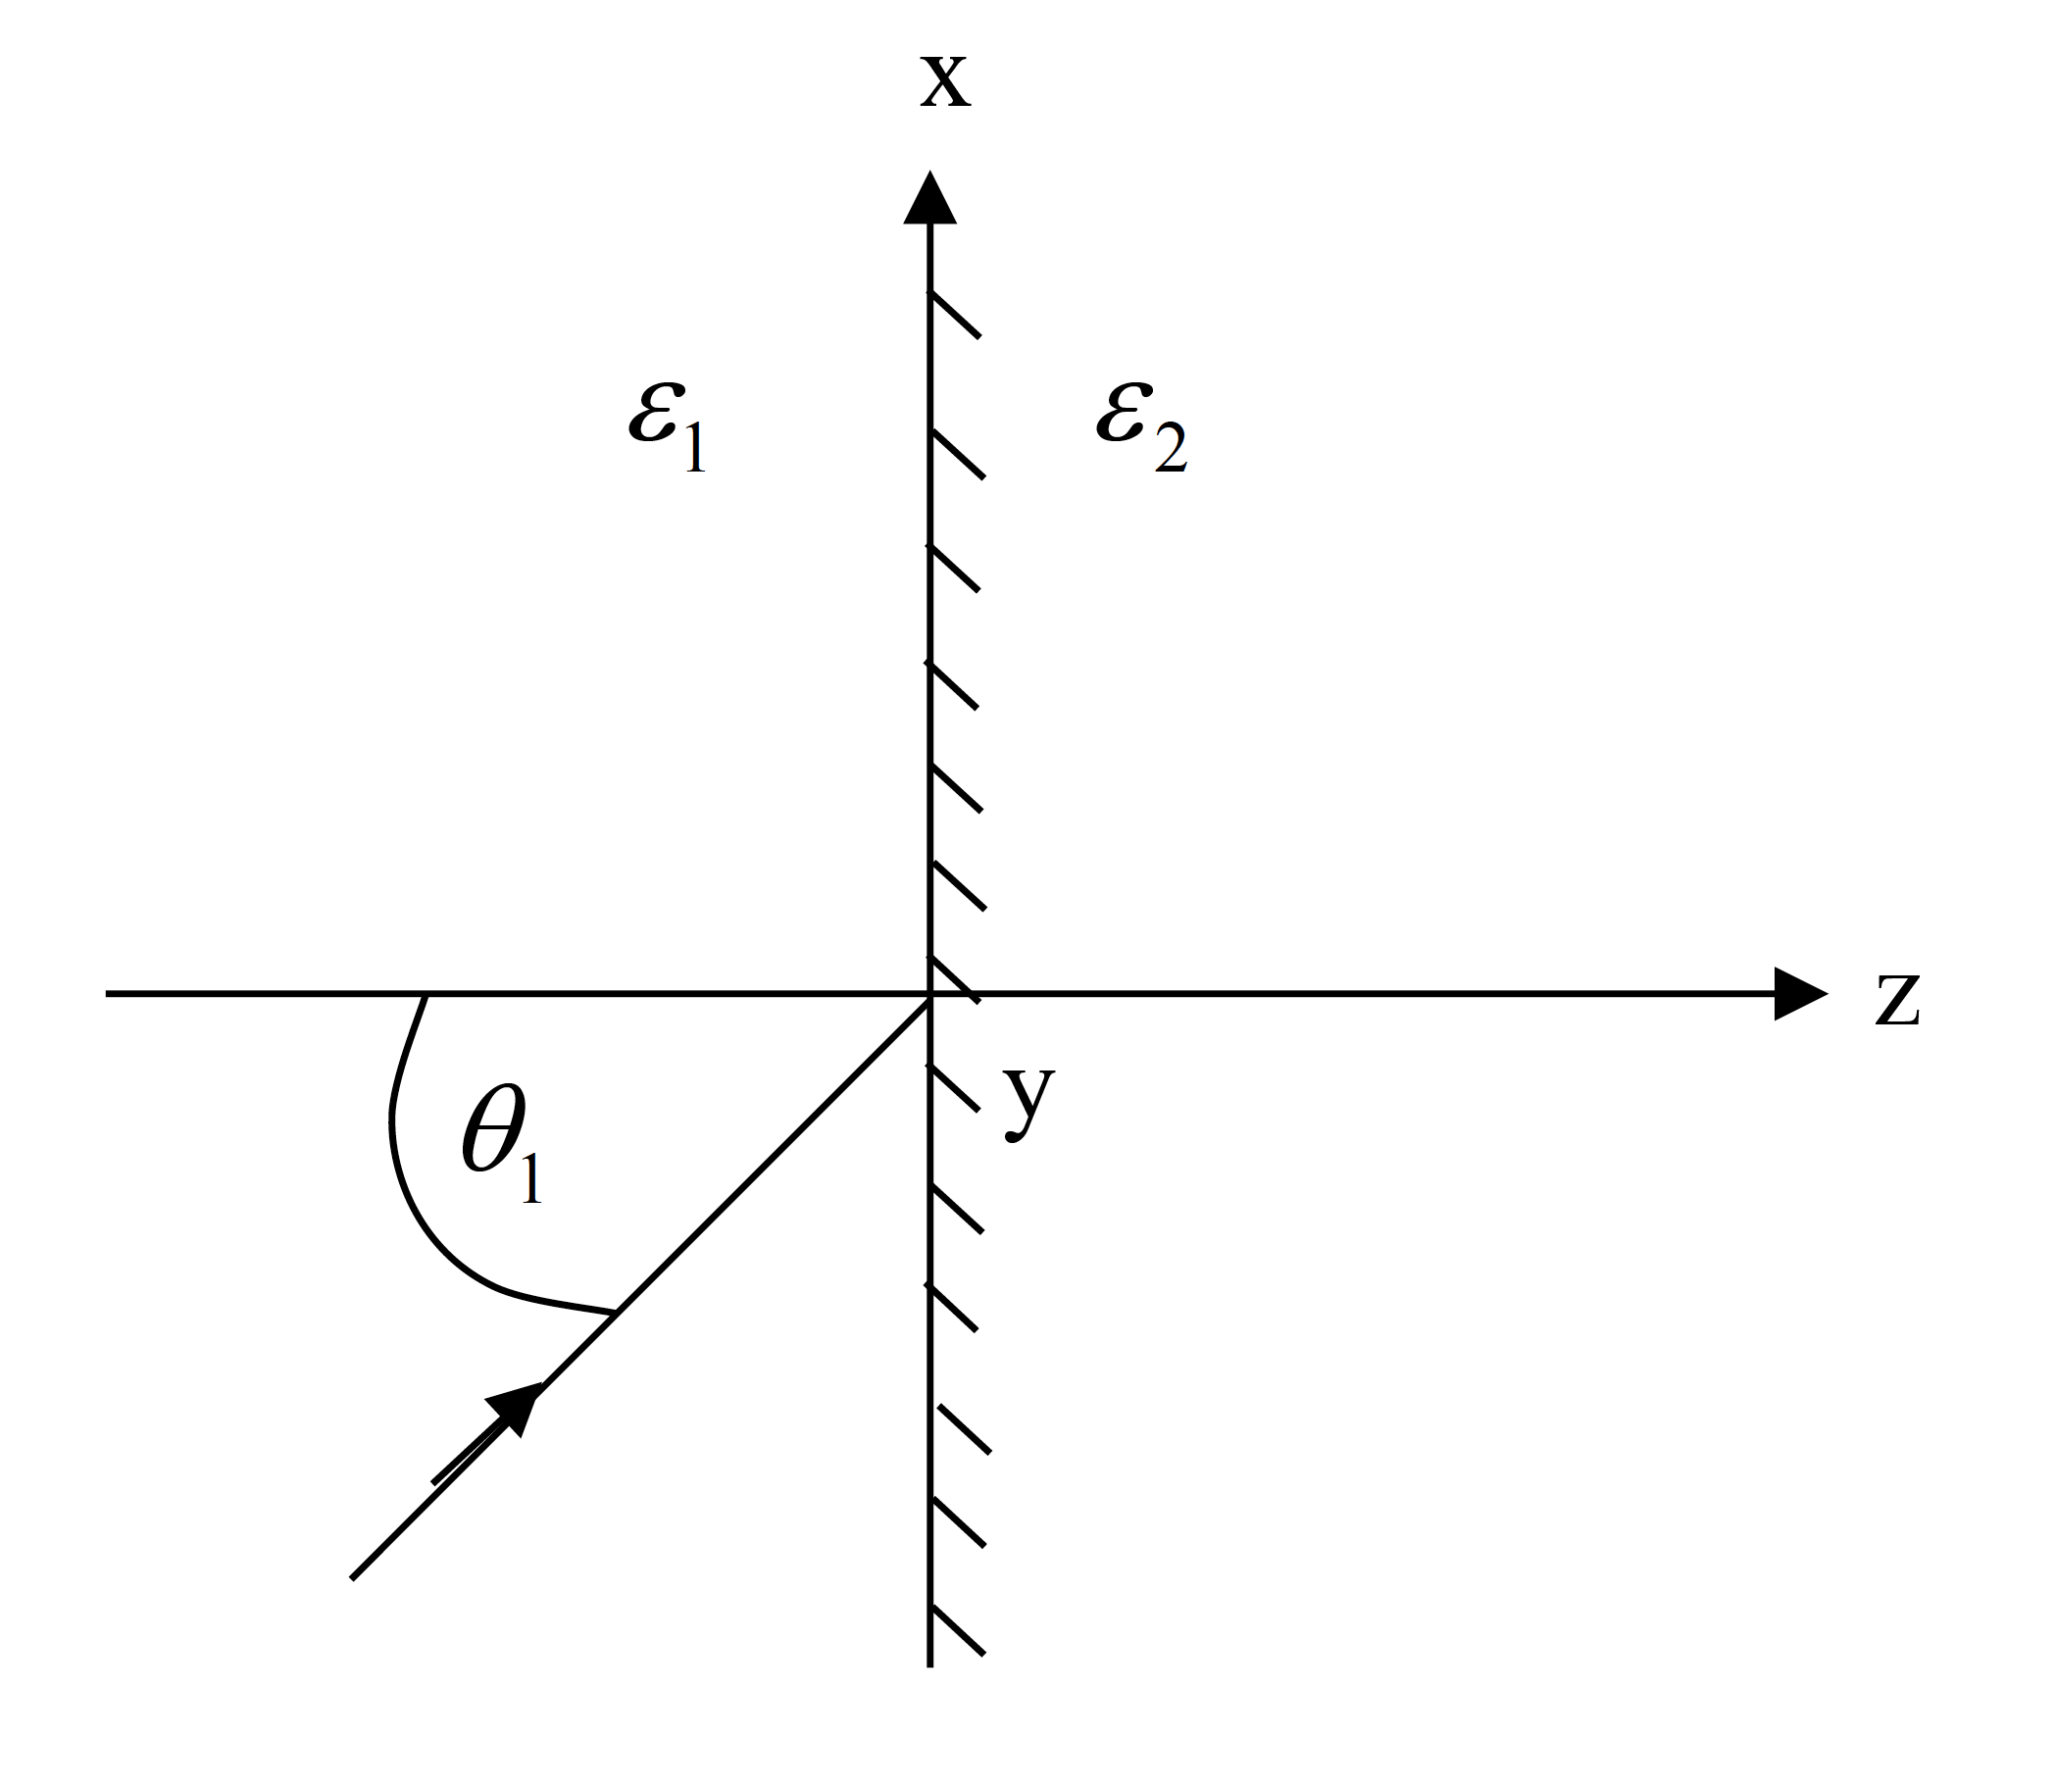
\includegraphics[width=3.0in]{2018spring/figures/12q_a.png}}
\caption{Plane wave incident in the interface between two dielectrics}
\label{fig:12q_a}
\end{figure}

    \begin{enumerate}
        \item \textbf{Q.} Find the angle $\theta_{1c}$ such that all waves incident with $\theta_1 > \theta_{1c}$ are "totally reflected". \textbf{Theory} In electromagnetism, the absolute permittivity, often simply called permittivity and denoted by the Greek letter $\varepsilon$ (epsilon), is a measure of the electric polarizability of a dielectric. The standard $\mathrm{SI}$ unit for permittivity is farad (unit of electrical capacitance) per meter $\left(\mathrm{F} / \mathrm{m}\right.$ or $\left.\mathrm{F} \cdot \mathrm{m}^{-1}\right)$

        $$
        \frac{\mathrm{F}}{\mathrm{m}}=\frac{\mathrm{C}}{\mathrm{V} \cdot \mathrm{m}}=\frac{\mathrm{C}^2}{\mathrm{~N} \cdot \mathrm{m}^2}=\frac{\mathrm{C}^2 \cdot \mathrm{s}^2}{\mathrm{~kg} \cdot \mathrm{m}^3}=\frac{\mathrm{A}^2 \cdot \mathrm{s}^4}{\mathrm{~kg} \cdot \mathrm{m}^3}
        $$
                
        The critical angle is the angle of incidence above which total internal reflection occurs. Total internal reflection occurs when light travels from a medium with a higher index of refraction to one with a lower index of refraction, and the angle of incidence is greater than the critical angle 1. The critical angle can be calculated using Snell's law, which states that $n_1 \sin \theta_1=n_2 \sin \theta_2$. When the incident angle equals the critical angle $\left(\theta_1=\theta_{1 c}\right)$, the angle of refraction is $90^{\circ}\left(\theta_2=90^{\circ}\right)$. Noting that $\sin 90^{\circ}=1$, Snell's law in this case becomes $n_1 \sin \theta_{1 c}=n_2$. \textbf{A.} A uniform plane wave is obliquely incident on the planar boundary between two semi-infinite material regions. 
        
        $$
        \theta^r=\theta^i
        $$
        
        i.e., angle of reflection equals angle of incidence. The refractive index of electromagnetic radiation equals
        
        $$
        n=\sqrt{\varepsilon_{\mathrm{r}} \mu_{\mathrm{r}}},
        $$
        
        where $\varepsilon_{\mathrm{r}}$ is the material's relative permittivity, and $\mu_{\mathrm{r}}$ is its relative permeability. The relative permittivity (in older texts, dielectric constant) is the permittivity of a material expressed as a ratio with the electric permittivity of a vacuum. In electromagnetism, permeability is the measure of magnetization produced in a material in response to an applied magnetic field. From Snell's law $n_1 \sin \theta_1=n_2 \sin \theta_2$:
        
        $$
        \sqrt{\mu_{r 1} \epsilon_{r 1}} \sin \theta^i=\sqrt{\mu_{r 2} \epsilon_{r 2}} \sin \theta^t
        $$
        
        where "$r$" in the subscripts indicates the relative (unitless) quantities. The associated formula for $\theta^t$ explicitly is:
        
        $$
        \theta^t=\arcsin \left(\sqrt{\frac{\mu_{r 1} \epsilon_{r 1}}{\mu_{r 2} \epsilon_{r 2}}} \sin \theta^i\right)
        $$
        
        When $\mu_{r 1} \epsilon_{r 1} > \mu_{r 2} \epsilon_{r 2}, \theta^t>\theta^r$; i.e., the transmitted wave appears to bend away from the surface normal. In fact, $\theta^t$ can be as large as $\pi / 2$ (corresponding to propagation parallel to the boundary) for angles of incidence which are less than $\pi / 2$. What happens if the angle of incidence is further increased? When calculating $\theta^t$, one finds that the argument of the arcsine function becomes greater than 1. Since the possible values of the sine function are between -1 and +1 , the arcsine function is undefined. Clearly our analysis is inadequate in this situation. To make sense of this, let us begin by identifying the threshold angle of incidence $\theta_c^i$  From the analysis in the previous paragraph,
        
        $$
        \sqrt{\frac{\mu_{r 1} \epsilon_{r 1}}{\mu_{r 2} \epsilon_{r 2}}} \sin \theta_c^i=1
        $$
        
        therefore,
        
        $$
        \theta_c^i=\arcsin \sqrt{\frac{\mu_{r 2} \epsilon_{r 2}}{\mu_{r 1} \epsilon_{r 1}}}
        $$
        
        This is known as the critical angle. When $\theta^i<\theta_c^i$, our existing theory applies. When $\theta^i \geq \theta_c^i$, the situation is, at present, unclear. For non-magnetic materials, the equation simplifies to
        
        $$
        \theta_c^i=\arcsin \sqrt{\frac{\epsilon_{r 2}}{\epsilon_{r 1}}}
        $$

        When the angle of incidence $\theta^i$ exceeds the critical angle $\theta_c^i$, the magnitude of the reflection coefficient is 1. In this case, all power is reflected, and no power is transmitted into the second medium. This is total internal reflection.
        
        \item \textbf{Q.} For $\theta_1 > \theta_{1c}$, describe the field (if any) in the region $z > 0$ in the $\varepsilon_2$ dielectric. \textbf{A.} As seen above for $\theta_1>\theta_c \rightarrow$ all wave will be reflected back in medium 1. So, there is no field inside the medium 2.

        \begin{figure}
        \centering\fbox{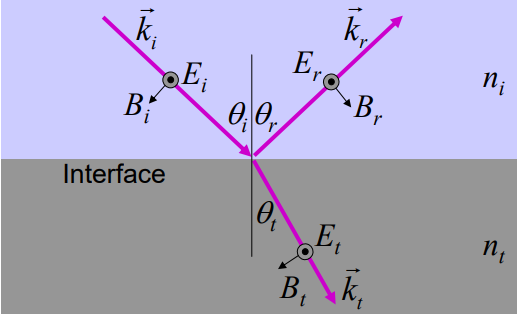
\includegraphics[width=3.0in]{2018spring/figures/12s_a.png}}
        \caption{S Polarization}
        \label{fig:12s_a}
        \end{figure}
        
        \item \textbf{Q.} If \underline{$E$} is perpendicular to the plane of the incidence, $\underline{E} = E_y \hat{y}$, find the phase of the reflection coefficient. \textbf{A.} $xz$ is the plane of incidence, and $xy$ is the plane of interface. S polarization is the perpendicular polarization, and the $E$ field sticks up out of the plane of incidence. P polarization is the parallel polarization, and $E$ field lies parallel to the plane of incidence. In this problem we have S polarization where the E-field is in Y axis. The intrinsic impedances of medium 1 and 2 are

        $$
        \begin{aligned}
        \eta_1 & =\sqrt{\frac{\mu_1}{\epsilon_1}} \\
        \eta_2 & =\sqrt{\frac{\mu_2}{\epsilon_2}}
        \end{aligned}
        $$
        
        The total electric E field is
        
        $$
        E_i(z=0)+E_r(z=0)=E_{t}(z=0).
        $$
        
        The total magnetic H field is
        
        $$
        -H_i(z=0) \cos \theta_i+ H_r(z=0) \cos \theta_r = -H_t(z=0) \cos \theta_t.
        $$
        
         where we know the $H$ field signs due to the right hand rule relationship between the pointing vector $\mathbf{k}$ (thumb), $E$ field (index) and $H$ (middle) field. We knows that
        
        $$
        \frac{E}{H}=\eta \text { so } \Rightarrow \eta_i=\frac{E_i}{H_i} ; \eta_r=\frac{E_r}{H_r} \text {; and } \eta_t=\frac{E_t}{H_t}
        $$
        
        so
        
        $$
        \begin{aligned}
        -\frac{E_i}{\eta_i} \cos \theta i+\frac{E_r}{\eta_r} \cos \theta_r &=-\frac{E_t}{\eta_t} \cos \theta_t \\
        &=-\frac{E_r+E_i}{\eta_t} \cos \theta_t \\
        &=-\frac{E_r}{\eta_t} \cos \theta_1-\frac{E_i}{\eta_t} \cos \theta_t \\
        \frac{E_r}{\eta_r} \cot \theta_r+\frac{E_r}{\eta_t} \cos \theta t &= \frac{E_i}{\eta_i} \cos \theta_i-\frac{E_i}{\eta_t} \cos \theta_t
        \end{aligned}
        $$
        
         We can relabel the impedances and angles because the incident and reflected wave are in the same medium and because the incident and reflected angles are the same
        
        $$
        \begin{aligned}
        \eta_r=\eta_i&=\eta_1\\
        \eta_t &= \eta_2 \\
        \theta_i &= \theta_r\\
        E_r\left[\frac{1}{\eta_1} \cos \theta_r+\frac{1}{\eta_2} \cot \theta_t\right] &= E_i\left[\frac{1}{\eta_i} \cos \theta_i - \frac{1}{\eta_2} \cos \theta_t\right]
       
        \end{aligned}
        $$

        Admittance is defined as
        
        $$
        Y \equiv \frac{1}{Z} \equiv \frac{1}{\eta}
        $$
        
        where $Y$ is the admittance, measured in siemens, and $Z$ is the impedance, measured in ohms.
    
        $$
        \frac{E_{y,r}}{E_{y,i}} = \frac{ Y_1 \cos \theta_i - Y_2 \cos \theta_t}{Y_1 \cos \theta_i + Y_2 \cos \theta_t}
        $$
        
        The refection coefficient in medium 1 is
        
        $$
        r_{\perp} = r_s = \frac{E_{y,r}}{E_{y,i}} =\frac{ Y_1 \cos \theta_i - Y_2 \cos \theta_t}{Y_1 \cos \theta_i + Y_2 \cos \theta_t}
        $$
        
        From here we can calculate phase and magnitude of the reflection coefficient.
    
    \end{enumerate}

\end{enumerate}
\end{document}